%%!TEX root = document.tex

Infectious diseases have substantial impact on health care, economics and society. 
Observational data might not be fully predictive for future outbreaks in adapted populations or settings and experiments in the real world process can have practical, budgetary or ethical constraints. Therefore, simulations and surrogate modeling can be very useful to mimic real world process and to inform policy makers on the prevention of infectious diseases and to obtain insights in transmission dynamics.

Our aim is to apply our CRSE tool to the input-output data of a computationally intensive high-performance simulator, STRIDE \citep{stride}, which models the transmission of infectious diseases.
The simulator is calibrated for measles outbreaks in Antwerp, a city in Belgium, with a population size of 500000 individuals. Of vital importance here is the population immunity aspect and as such, our research question is: how does the immunization fraction influence the outbreak of measles?
In this paper, we focus on the convergence characteristics of the surrogate models rather than their domain specific implications. 

A single simulation run with this individual-based model is computationally expensive hence surrogate models, approximating the detailed simulator, can be useful as an emulator to improve model exploration and facilitate rapid policy making in various settings. 
Symbolic regression can be used to obtain surrogate models based on input-output simulation data. Generating all simulation output in sequence prior to building the surrogate model leads to significant downtime for the user. 
Therefore, we elaborate on the value of an incremental approach with surrogate models based on partial results of the simulation model with the aim to setup a trustworthy feedback loop between the user, simulator and regression tool. 
This incremental approach provides partial results to a domain expert to enhance the model building and design of experiments. Our CRSE tool is able to reuse partial results to seed subsequent runs. %We elaborate in this section whether this approach can lead to improved models.

% please, limit the number of abbreviations to increase the readability for your audience
\paragraph{Design of experiment}
To run the disease transmission simulator, we used a space filling design to maximize the sampling of the parameter space and minimize the number of evaluation points. We applied a Latin Hypercube Design, specifically the Audze-Eglais \citep{AudzeEglais, AudzeEglais2, AudzeEglais3}, which uses the Euclidean distance measure but in addition obtains a uniform distribution of the individual points. This design relies on the concept of minimizing a potential energy between design points, a measure based on the inverse of the euclidean distance.
\[
E^{AE} = \sum_{i=0}^{p-1} {\sum_{j=i+1}^{p-1} {\frac{1}{d_{ij}}}}
\]

%\paragraph{Simulator configuration}
We constructed an experimental design with 3 dimensions and 30 points, using the tool introduced by Husslange et al. \citep{DOE}, for the following parameters:
\begin{itemize}
\item Basic reproduction number (R$_0$) : the expected number of secondary infections caused by a primary infection in a fully susceptible population, [12-20]
\item Starting set of infected persons (S) : Number of persons in the population that is an infected person at the start of the simulation, [1-500]
\item Immunity fraction (I) : Fraction of the population that is immune to the disease at the start of the simulation. [0.75, 0.95]
\end{itemize}
For each parameter we used 30 points uniformly chosen in their range and each configuration is used to run the disease simulator once. 
We used the the attack rate as output parameter, which is the rate of the total number of cases in the population versus the size of the population. 



\paragraph{Symbolic regression configuration}
We run the GP-SR with 30 phases, each consisting of 60 generations of 20 expressions with an initial depth of 3 and maximum depth of 6. The 4 best expressions of each phase are archived. %LW: why 4 here and 5 in the previous section?
We compare 3 approaches based on fitness and computational cost. Firstly, we run all 30 configurations and use the CSRM tool on the entire simulation dataset. This is the traditional approach where the GP-SR tool starts a blind search and serves as baseline in our comparisons.
Secondly, we split the configurations into incremental sections. We start the CSRM tool with the results from 10 configurations. The best 4 results are saved to disk and used to seed the GP-SR with  20 simulated configurations. The results of the 20-point dataset are used to seed for the 30-point CSRM run. The computational cost of analyzing 10-, 20-, or 30-point simulation output is similar. 
Thirdly, we run the tool on the data from 30 configurations with a double amount of phases. As such, the same number of fitness evaluations are performed as with the 10-20-30 combination. 
We run the experiment distributed to observe the change in convergence characteristics using the seeds of the 10-20-30 combination to combine the distributed and incremental features of our tool. %LW: please rephrase...

%\subsection{Results}
\subsubsection{Fitness improvement}
We compare the seeded and extended CSRM runs with the baseline 30-point run.  Figure \ref{fig:incrementalgain} shows that the fitness, accuracy to predict the response, improved for the training data for all methods. For the valuation data, we observed that the "20-point analysis seeded by the 10-point run" performs worse compared to the blind search on the full output. As such, 2/3rd of the simulations seems not enough, leading to overfitting. If we seed the best results from the 20-point CSRM run into a 30-point configuration, we observed that both the training and validated fitness values substantially improved. The 30-point CSRM run with 60 phases has the same computational cost as the combined 10-20-30 analysis, but has only little to no gain in convergence by the additional phases. We see that convergence is slowing, with training fitness improving by a factor of 10 \%, but validation fitness worsens. %LW: please rephrase...
This is a typical example of overfitting. The combined 10-20-30 run increases validation fitness with a factor of 13\%

\subsubsection{Distributed}
We performed the 10-20-30 analysis also in the distributed setting and compared the topologies in terms of fitness improvement and speed-up. We used 25 processes in a Tree, Grid and Random and   Disconnected topology. Figure \ref{fig:usecasedistributed} presents the gain in fitness on the validation data for the Tree, Grid and Random topologies compared to the Disconnected topology. We observed that the diffusion in the Grid topology leads to the highest gain, followed by the Tree topology. Interestingly, the Random topology scored less than the Disconnected topology. This can occur when an early local optimum dominates the remainder of the process. The effect on runtime is showed in Figure \ref{fig:usecasespeedup}, with the Tree topology encountering minimal overhead. The Grid topology has a performance penalty of factor 2 and the Random topology performed intermediate. During the experiments, we observed that the progress of the processes in the Tree and Disconnected topologies could vary up to 4 phases. This can be explained by the distance between two processes in the Tree topology, which is at most 4 (depth of a 25-node binary tree). As such, if we increase the number of processes in the Tree topology, it will scale better. %The delay tolerance allows the tree topology this scaling effect.

\begin{figure}
    \begin{subfigure}{0.5\textwidth}
        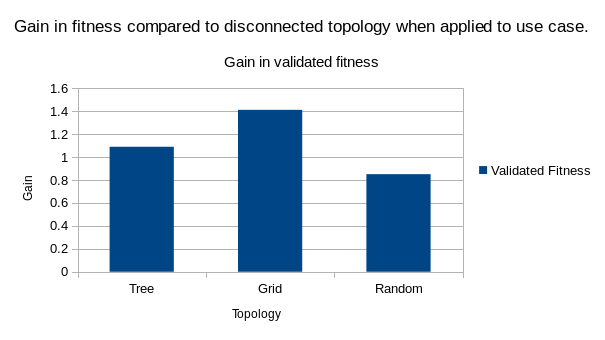
\includegraphics[width=0.8\linewidth]{figures/usecasedistributed.png}
		\caption{Incremental distributed CSRM applied to use case.}
		\label{fig:usecasedistributed}
    \end{subfigure}
    \begin{subfigure}{0.5\textwidth}
        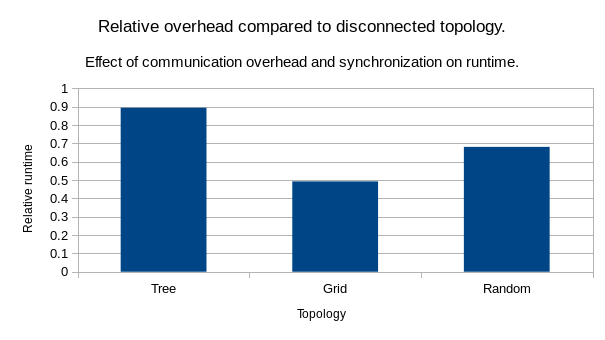
\includegraphics[width=0.8\linewidth]{figures/usecasespeedup.png}
		\caption{Runtime impact of synchronization and communication overhead.}
		\label{fig:usecasespeedup}
    \end{subfigure}
        \begin{subfigure}{0.5\textwidth}
        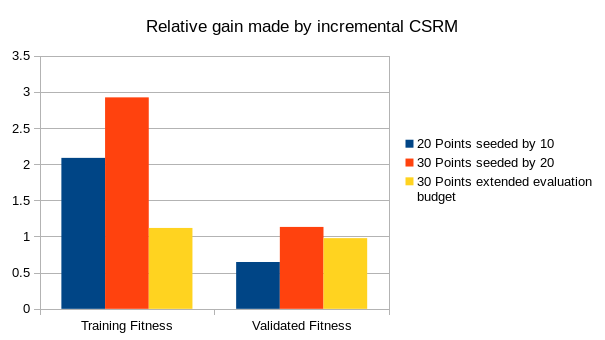
\includegraphics[width=0.8\linewidth]{figures/incrementalgain.png}
        \caption{Incremental fitness gain in CSRM.}
        \label{fig:incrementalgain}
    \end{subfigure}
        \begin{subfigure}{0.5\textwidth}
        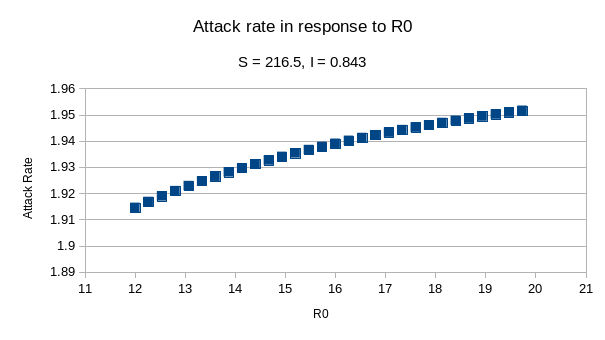
\includegraphics[width=0.5\linewidth]{figures/responseR.png}
        \caption{Response of attack rate to R.}
    \end{subfigure}
    \begin{subfigure}{0.5\textwidth}
        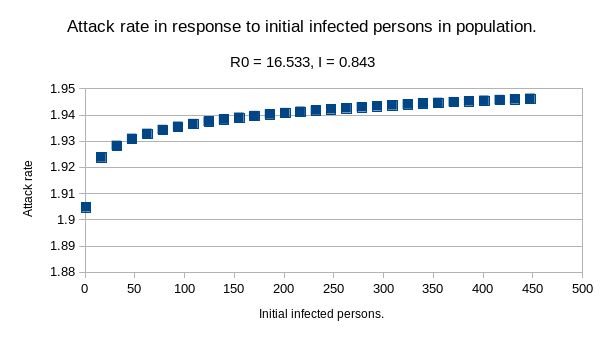
\includegraphics[width=0.5\linewidth]{figures/responseS.png}
        \caption{Response of attack rate to S.}
    \end{subfigure}
        \begin{subfigure}{0.5\textwidth}
        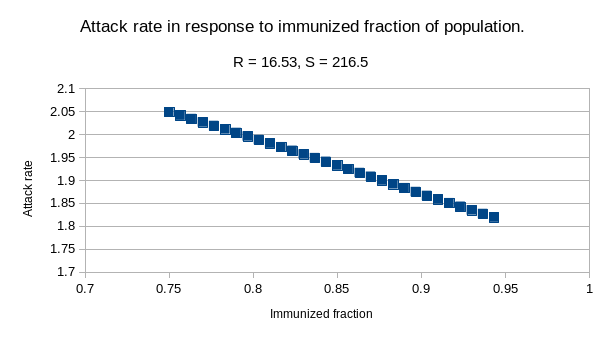
\includegraphics[width=0.5\linewidth]{figures/responseI.png}
        \caption{Response of attack rate to I.}
        \label{fig:usecaseresponseplots}
    \end{subfigure}
    %\caption{Use case : Effect of topology on fitness correlation of distributed processes.}
    %\label{fig:usecasecorrelation}
\end{figure}

Based on runtime and scaling, we obtained the best results with the distributed application of CSRM with a Tree topology. This resulted in an algebraic expression with a fitness value of 0.039 on the full data set. However, it is still 10 orders of magnitude removed from the optimal prediction of the response, which is an indication of the value that partial results can offer. 
The effect of each parameter on the response can be explored using response plots. As such, we vary each of the parameters while keeping the others fixed to the midpoint of the range, and calculate an estimate of the attack rate. We observed that our surrogate model predicts an attack rate outside of the valid range of [0,1]. This might be explained by the scaling factor of 10 between the prediction and the actual output from the simulator. The surrogate models from the CSRM tool are trained with 30 data points and not the full factorial design. Nonetheless, the response plots can be used to evaluate points that were not available in our trading set. The trends in the response plots are in line with the literature [REF 13].  R$_0$ increases logarithmic with the attack rate, which is in line with theoretical and empirical results. An increasing trend is also observed with the initial number of infected persons. An in crease in the immunization fraction shows a decease in the predicted attack rate. While the exact values of the predicted attack rate from our suboptimal surrogate model are not yet correctly, the expected trends are. This justify our incremental approach since surrogate models will  match the trend first, rather than fitting individual points. This can be partly explained by our usage of the Pearson R correlation coefficient as basis for the fitness function. 

